\documentclass{standalone}
\usepackage{tikz}
\usetikzlibrary{decorations.pathmorphing}

\begin{document}
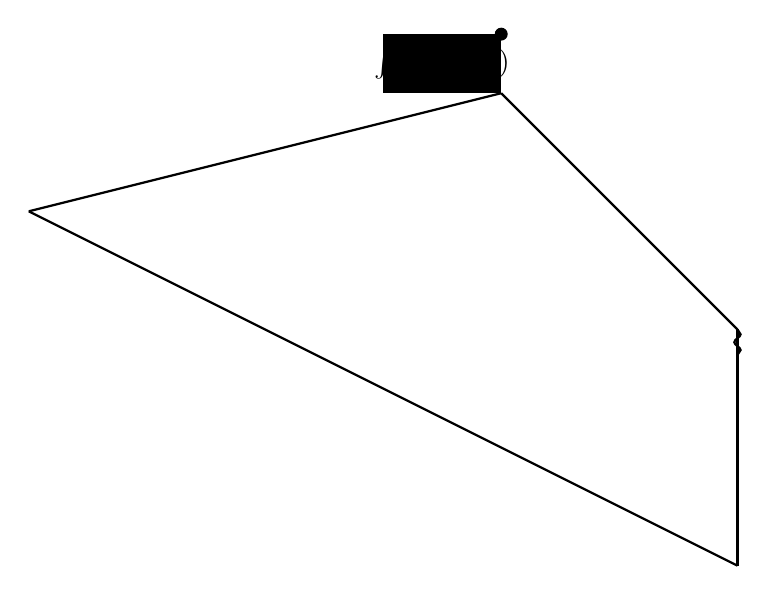
\begin{tikzpicture}[scale=1.5]
    % Draw the right boundary line
    \draw[thick] (0,0) -- (0,2);
    \draw[thick] (0,2) -- (-2,4);
    \draw[thick] (-2,4) -- (-6,3);
    \draw[thick] (-6,3) -- (0,0);

    % Highlight the area of interest with a filled black segment and label
    \fill[black] (-2,4) -- (-2,4.5) -- (-3,4.5) -- (-3,4) -- cycle;
    \node at (-2.5,4.25) {$\int dx O(x,t)$};

    % Add a wavy line to represent the asymptotic boundary
    \draw[decorate,decoration={snake,amplitude=.4mm,segment length=2mm,post length=1mm},thick] (0,2) -- ++(0,-0.3);

    % Add a small dot at the endpoint of the highlighted area
    \filldraw[black] (-2,4.5) circle (0.05);
\end{tikzpicture}
\end{document}